% AUTHOR: M. CAN KANDEMIR
% CONTACT: cnkndmr@gmail.com

\documentclass[aspectratio=1610]{beamer}
\usepackage[utf8]{inputenc}
\usetheme{Madrid}
\usecolortheme{beaver}
\usepackage{graphicx}
\graphicspath{ {./figures/} }
\usepackage{wrapfig}
\usepackage{multicol}
\usepackage{multirow}
\usepackage{array}
\usepackage{caption}
\usepackage{amsmath,amsthm, amssymb, latexsym}
\setbeamertemplate{navigation symbols}{}
\setbeamerfont{caption}{size=\scriptsize}
\setbeamertemplate{caption}[numbered]
\renewcommand{\arraystretch}{1.2}
\title[Molecular Docking]
{DNA interaction of some hydantoin-based drugs \newline with molecular docking calculations}

\author[M. Can Kandemir (I.U.)]
{M. Can Kandemir$^{1}$, Aslan Saları$^{1}$,\\Bilge Bıçak$^{1}$, and Serda K. Gündüz$^{1,*}$}

\institute[]
{
	\textbf{1:} Physics Department, Science Faculty, Istanbul University,\\Vezneciler, 34134, Istanbul, Turkey
	\and
	\textbf{*:} skecel@istanbul.edu.tr
}

\date[TPS35]
{Turkish Physical Society 35$^{th}$\newline International Physics Congress}

\begin{document}
	\begin{frame}
		\vspace{0.4em}
		
\includegraphics[height=5em]{Istanbul_Universitesi.png}
		\hfill
		
\includegraphics[height=5em]{Istanbul_Universitesi_Fen.png}
		\titlepage
	\end{frame}
	\begin{frame}
		\frametitle{Abstract}
%\centering
Drug-DNA interactions are very important in pharmaceutical chemistry because drug interactions of anticancer, antiviral, antibacterial and other drugs are directly related to their binding to DNA. In this study, molecular docking calculations were performed to investigate B-DNA dodecamer d(CGCGAATTCGCG) binding interaction with hydantoin-based drugs such as Phenytoin, Mephenytoin, and Ethotoin. According to the results of molecular docking, the interaction area and binding distances between the three drugs and DNA helix were determined. The results show that Phenytoin and Ethotoin bound to DNA with -5.8 kcal/mol binding energies, Mephenytoin bound to DNA with -6.0 kcal/mol binding energies respectively. B-DNA dodecamer (PDB: 1BNA) with 1.9 Å resolution was used for docking calculations in order to investigate the drug binding area with binding energies. Molecular docking calculations were realized using AutoDock 4.2 software.
	\end{frame}
	\begin{frame}
		\frametitle{Epilepsy and Antiepileptic drugs}
\par As a definition, epilepsy is the name of a brain disorder characterized predominantly by recurrent and unpredictable interruptions of normal brain function \cite{fisher2005epileptic}. It affects people from both sexes and all ages. Approximately 50 million people worldwide have this neurological disorder \cite{world2006neurological}. It is characterized by repeated seizures, which are brief episodes of uncontrolled movement that may involve a part of the body (partial) or the entire body (generalized) and sometimes followed by loss of consciousness and control of bowel or bladder function. Mostly reasons of epileptic seizures are excessive and abnormal neuronal activity in the cortex of the brain \cite{fisher2005epileptic}. Seizure episodes result from excessive electrical discharges in a group of brain cells. Different parts of the brain can be the site of such discharges.
\newline
\par Antiepileptic drugs (AEDs) are used to prevent epileptic seizures. AEDs (such as Phenytoin, Mephenytoin, and Ethotoin) are a diverse group of pharmacological agents used in the treatment of epileptic seizures. AEDs suppress the excessive rapid discharge of neurons during seizures. AEDs also prevent the spread of the seizure within the brain. Seizures can be controlled up to 70\% of people living with epilepsy could become seizure free with use of antiseizure medications \cite{sander1993some}.
	\end{frame}
	\begin{frame}
		\frametitle{Phenytoin}
\begin{columns}
\begin{column}{0.6\linewidth}
	Phenytoin (C$_{15}$H$_{12}$N$_{2}$O$_{2}$, Dilantin) is a major antiepileptic drug (AED).
	Structure of phenytoin is a imidazolidine-2,4-dione that consists of hydantoin bearing two phenyl substituents at position 5, respectively.
	It is the most used drug for major epilepsy and the treatment of partial and generalised seizures such as tonic-clonic seizures.
	It also use as an antiarrhythmic, muscle relaxant, teratogenic agent, and a sodium channel promoter.
	Mechanism of action of Phenytoin acts by promoting sodium efflux from neurons in the motor cortex, reducing post-tetanic potentiation at synapses.
	The 3D structure of Phenytoin obtained from ZINC database with code 1665626.
%	Phenytoin is a well known inducer of CYP3A4 \cite{nishibe1995induction}.
\end{column}
\begin{column}{0.4\linewidth}
	\begin{figure}
		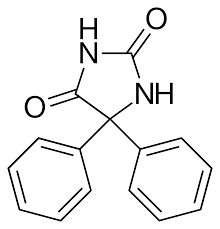
\includegraphics[width=0.8\linewidth]{phenytoin_str.png}
		\caption{\centering The structure of Phenytoin.}
		\label{fig:pht_str}
	\end{figure}
\end{column}
\end{columns}
	\end{frame}
	\begin{frame}
		\frametitle{Mephenytoin}
\begin{columns}
\begin{column}{0.6\linewidth}
	\par Mephenytoin (C$_{12}$H$_{14}$N$_{2}$O$_{2}$, Mesantoin) is an antiepileptic drug with a heterocyclic organic compound.
	Structure of mephenytoin is an imidazolidine-2,4-dione (hydantoin) in which the imidazolidine nucleus carries a methyl group at N-3 and has ethyl and phenyl substituents at C-5, respectively.
	Mechanism of action is, promotes sodium efflux from neurons in motor cortex, and stabilizes the threshold against hyperexcitability caused by excessive stimulation.
	Due to these properties, mephenytoin reduces the membrane sodium gradient and prevents cortical seizure signal spreading.
	The 3D structure of Mephenytoin obtained from ZINC database with code 453.
\end{column}
\begin{column}{0.4\linewidth}
	\begin{figure}
		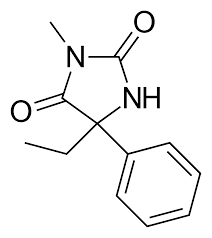
\includegraphics[width=0.8\linewidth]{mephenytoin_str.png}
		\caption{\centering The structure of Mephenytoin.}
		\label{fig:mph_structure}
	\end{figure}
\end{column}
\end{columns}
	\end{frame}
	\begin{frame}
		\frametitle{Ethotoin}
\begin{columns}
	\begin{column}{0.6\linewidth}
		\small
		Ethotoin (C$_{11}$H$_{12}$N$_{2}$O$_{2}$, Peganone) is a member of hydantoin derivative antiepileptic drug.
		Structure of ethotoin is an imidazolidine-2,4-dione that is hydantoin substituted by ethyl and phenyl at positions 3 and 5, respectively.
		Mechanism of action of ethotoin is, influences synaptic transmission by altering sodium and calcium ion influx across neuronal membranes in the repolarization, depolarization, and membrane stability phase and interferes with the calcium uptake in presynaptic terminals.
		This inhibits neuronal discharge and occurs in the stabilization of neuronal membranes, there by preventing the spread of seizure activity at the motor cortex.
		Ethotoin is also generally used for tonic-clonic and partial complex seizures.
		The 3D structure of Ethotoin obtained from ZINC database with code 271.
	\end{column}
	\begin{column}{0.4\linewidth}
		\begin{figure}
			
\includegraphics[width=0.7\linewidth]{ethotoin_str.png}
			\caption{\centering The structure of Ethotoin.}
			\label{fig:eth_structure}
		\end{figure}
	\end{column}
\end{columns}	
	\end{frame}
	\begin{frame}
		\frametitle{Docking Analysis}
Structure based computational modeling of ligand-receptor interactions is a prominent part of modern drug discovery. Molecular docking calculations are often preferred methods that used in the structure-based drug design (SBDD) studies to define the interaction of the molecule with the protein in which the molecule interacts within the body, respectively. Molecular docking study is also able to predict the binding conformations and free energies of ligands that is drug candidate molecules within the appropriate target binding site \cite{ferreira2015molecular}. Molecular docking calculations were realized using AutoDock Vina 1.1.2 \cite{trott2010autodock} software.
	\end{frame}
	\begin{frame}
		\frametitle{Receptor}
The B-DNA dodecamer d(CGCGAATTCGCG) described by James Watson and Francis Crick The double helix makes one complete turn about its axis every 10.4–10.5 base pairs in solution. This frequency of twist (termed the helical pitch) depends largely on stacking forces that each base exerts on its neighbours in the chain. \begin{wrapfigure}{r}{0.5\textwidth}
	\vspace{-2em}
	\begin{center}
		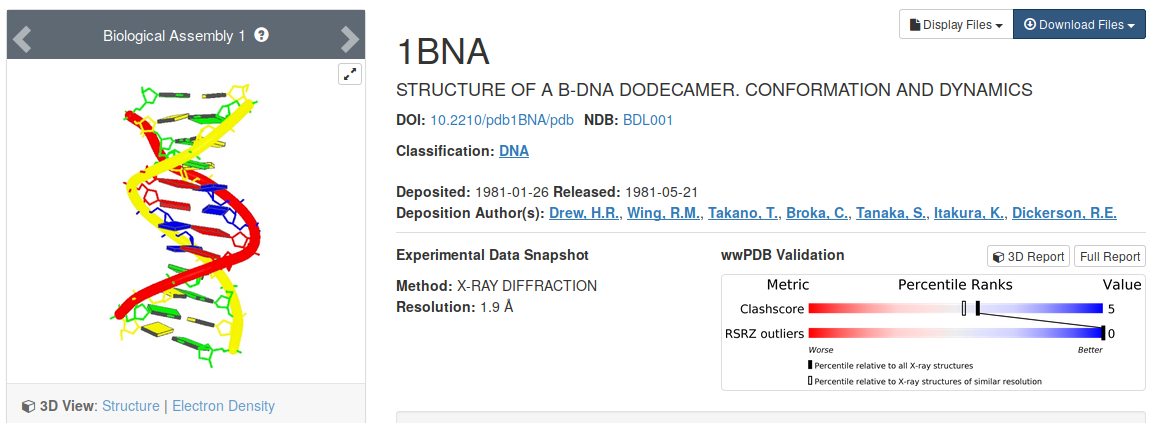
\includegraphics[width=0.5\textwidth]{receptor.png}
	\end{center}
\end{wrapfigure}The absolute configuration of the bases determines the direction of the helical curve for a given conformation. The 3D structure of a B-DNA dodecamer containing the atom count of 486 with the 1.9Å was obtained from the PDB (PDB: 1BNA) \cite{drew1981structure}.

	\end{frame}
	\begin{frame}
		\frametitle{Docking results of Phenytoin}
\begin{columns}
	\begin{column}{0.6\linewidth}
		\begin{figure}
			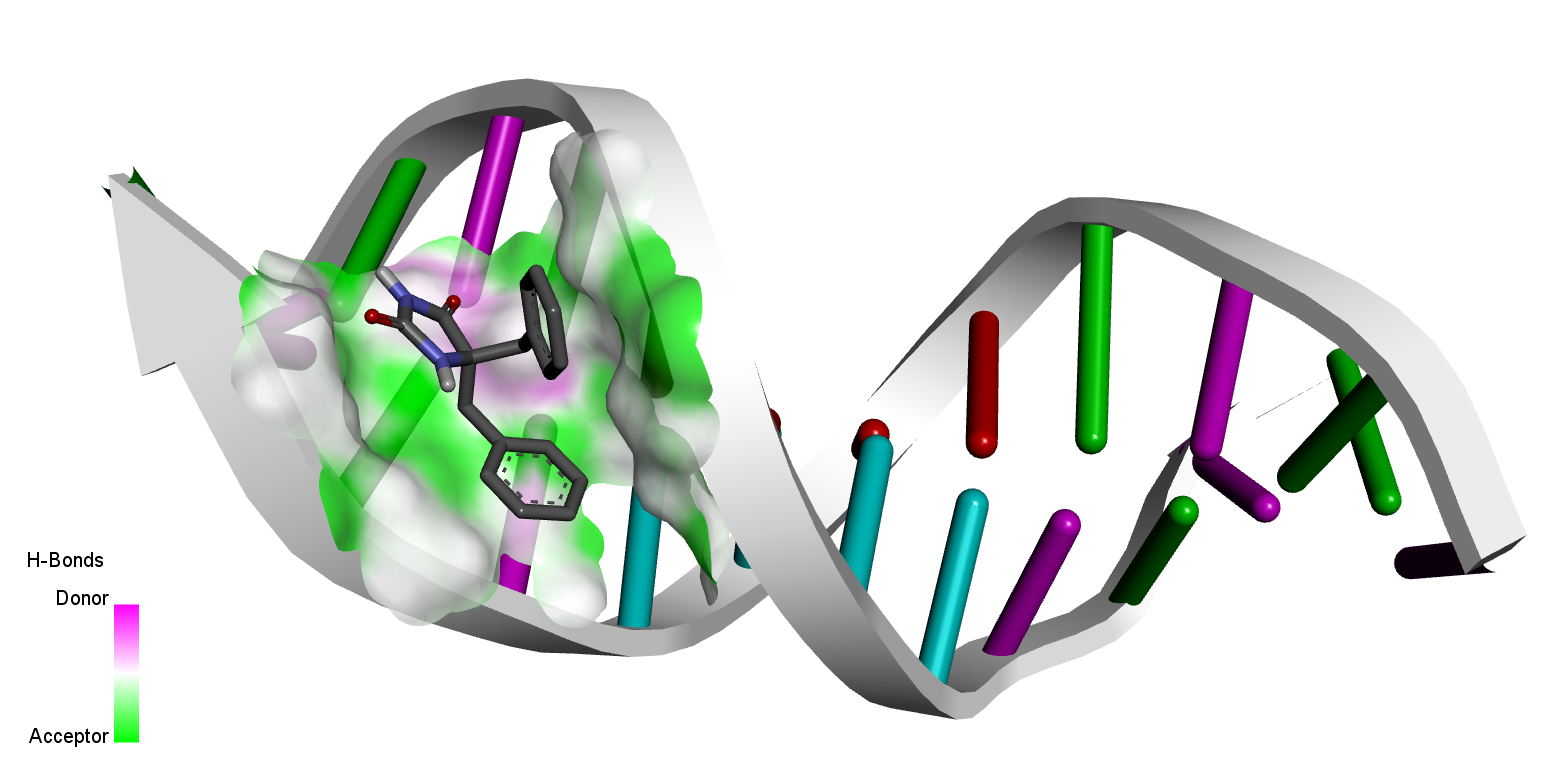
\includegraphics[width=\linewidth]{phenytoin-donor-acceptor.png}
			\caption{\centering The donor-acceptor interaction \linebreak between Phenytoin and B-DNA.}
			\label{fig:pht_donor_acceptor}
		\end{figure}
	\end{column}
	\begin{column}{0.45\linewidth}
		\centering
		\scriptsize
		\begin{table}
			\begin{tabular}{*{4}{c}}
				\hline\\[-1em]
				\multirow{2}{2em}{\centering\textbf{Mode}}&\multirow{2}{4em}{\centering\textbf{Affinity (kcal/mol)}}&\multicolumn{2}{c}{\centering\textbf{Distance from best mode}}\\
				\cline{3-4}
				&&\textbf{rmsd l.b.}&\textbf{rmsd u.b.}\\
				1&-5.8&0.000&0.000\\
				2&-5.7&2.433&3.604\\
				3&-5.7&2.081&5.276\\
				4&-5.7&2.863&4.281\\
				5&-5.5&2.633&3.968\\
				6&-5.5&2.360&3.522\\
				7&-5.4&1.717&2.503\\
				8&-5.4&2.296&4.480\\
				9&-5.3&2.010&3.798\\
				\hline
			\end{tabular}
			\caption{\centering The binding affinities and RMSD values between Phenytoin and B-DNA.}
			\label{table:pht}
		\end{table}
	\end{column}
\end{columns}
	\end{frame}
	\begin{frame}
		\frametitle{Docking results of Phenytoin}
\begin{columns}
	\begin{column}{0.5\linewidth}
		\centering
		\vspace{-1.5em}
		\begin{figure}
			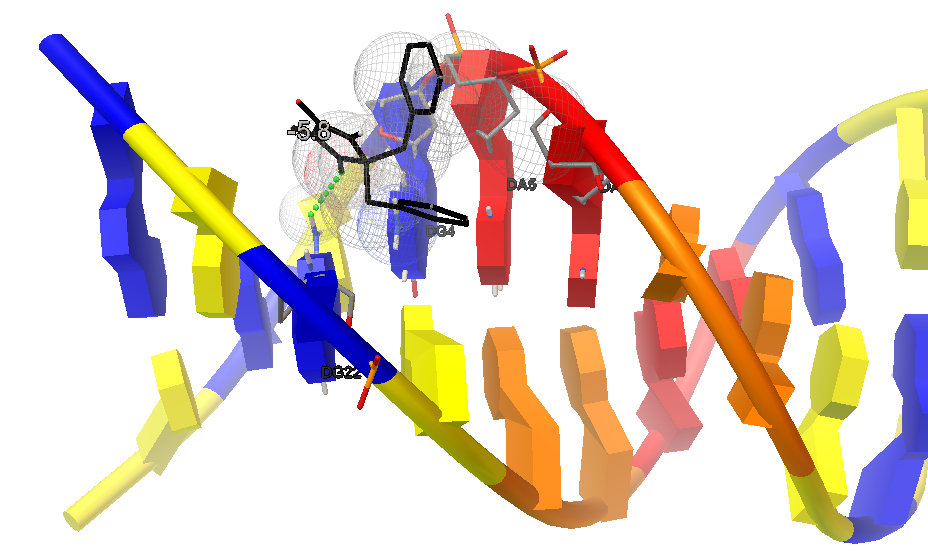
\includegraphics[width=0.8\linewidth]{phenytoin_ribbon_2.png}
			\caption{\centering The hydrogen bonding interaction \linebreak between Phenytoin and B-DNA.}
			\label{fig:pht_ribbon}
		\end{figure}
		\vspace{-2.5em}
		\tiny
		\begin{table}
		\begin{tabular}{ c | c c c } 
			\multirow{2}{7.6em}{\centering \textbf{Close interactions with B-DNA}}&\multicolumn{3}{c}{\multirow{2}{10em}{\centering DA5, DA6, DG22, DG4}}\\
			&&&\\
			\hline
			\multirow{8}{7em}{\centering \textbf{Hydrogen bonds (Angstrom Å) with B-DNA}}&\multirow{2}{6em}{\centering \textbf{Donor Atom}}&\multirow{2}{4em}{\centering \textbf{Acceptor Atom}}&\multirow{2}{5em}{\centering \textbf{Bond Length (Å)}}\\
			&&&\\
			\cline{2-4}
			&\multirow{2}{6em}{\centering H21 of DG22 (Chain B)}&\multirow{2}{6em}{\centering O2 of Phenytoin}&\multirow{2}{2em}{\centering 2.2}\\
			&&&\\
			\cline{2-4}
			&\multirow{2}{6em}{\centering H22 of DG4 (Chain A)}&\multirow{2}{6em}{\centering O2 of Phenytoin}&\multirow{2}{2em}{\centering 2.3}\\
			&&&\\
			\cline{2-4}
			&\multirow{2}{6em}{\centering H3 of DG4 (Chain A)}&\multirow{2}{6em}{\centering O2 of Phenytoin}&\multirow{2}{2em}{\centering 3.2}\\
			&&&\\
		\end{tabular}
		\caption{\centering{The close and hydrogen bonds \linebreak between Phenytoin and B-DNA.}}
		\end{table}
	\end{column}
	\begin{column}{0.5\linewidth}
		\centering
		\scriptsize
		\begin{figure}
			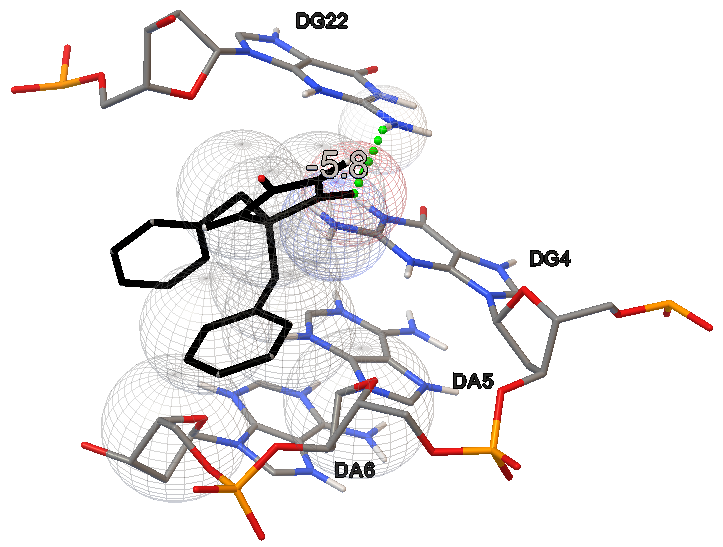
\includegraphics[width=\linewidth]{phenytoin_yakin_1.png}
			\caption{\centering The close interaction and
				binding affinity \linebreak between Phenytoin and B-DNA.}
			\label{fig:phe_close}
		\end{figure}
	\end{column}
\end{columns}
	\end{frame}
	\begin{frame}
		\frametitle{Docking results of Mephenytoin}
\begin{columns}
	\begin{column}{0.6\linewidth}
		\begin{figure}
			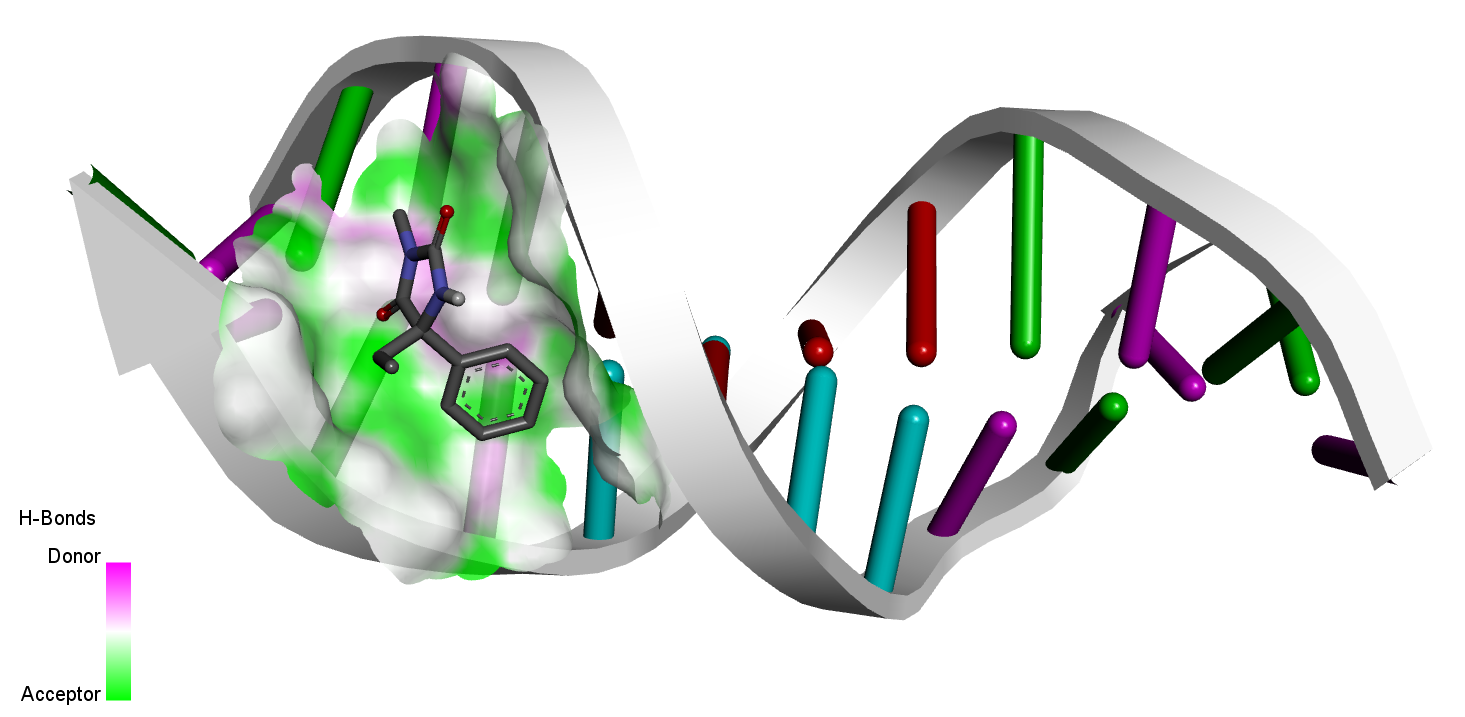
\includegraphics[width=\linewidth]{mepheytoin-donor-acceptor.png}
			\caption{\centering The donor-acceptor interaction \linebreak between Mephenytoin and B-DNA.}
			\label{fig:mph_donor_acceptor}
		\end{figure}
	\end{column}
	\begin{column}{0.45\linewidth}
		\centering
		\scriptsize
		\begin{table}
			\begin{tabular}{*{4}{c}}
				\hline\\[-1em]
				\multirow{2}{2em}{\centering\textbf{Mode}}&\multirow{2}{4em}{\centering\textbf{Affinity (kcal/mol)}}&\multicolumn{2}{c}{\centering\textbf{Distance from best mode}}\\
				\cline{3-4}
				&&\textbf{rmsd l.b.}&\textbf{rmsd u.b.}\\
				1&-6.0&0.000&0.000\\
				2&-6.0&0.225&1.217\\
				3&-5.9&2.588&4.660\\
				4&-5.6&1.942&2.857\\
				5&-5.4&1.453&1.985\\
				6&-5.3&2.002&4.710\\
				7&-5.2&1.916&5.436\\
				8&-5.1&2.079&4.524\\
				9&-5.0&2.357&3.786\\
				\hline
			\end{tabular}
			\caption{\centering The binding affinities and RMSD values between Mephenytoin and B-DNA.}
			\label{table:mph}
		\end{table}
	\end{column}
\end{columns}
	\end{frame}
	\begin{frame}
		\frametitle{Docking results of Mephenytoin}
\begin{columns}
%	\hspace{em}
	\begin{column}{0.5\linewidth}
		\centering
		\vspace{-1em}
		\begin{figure}
			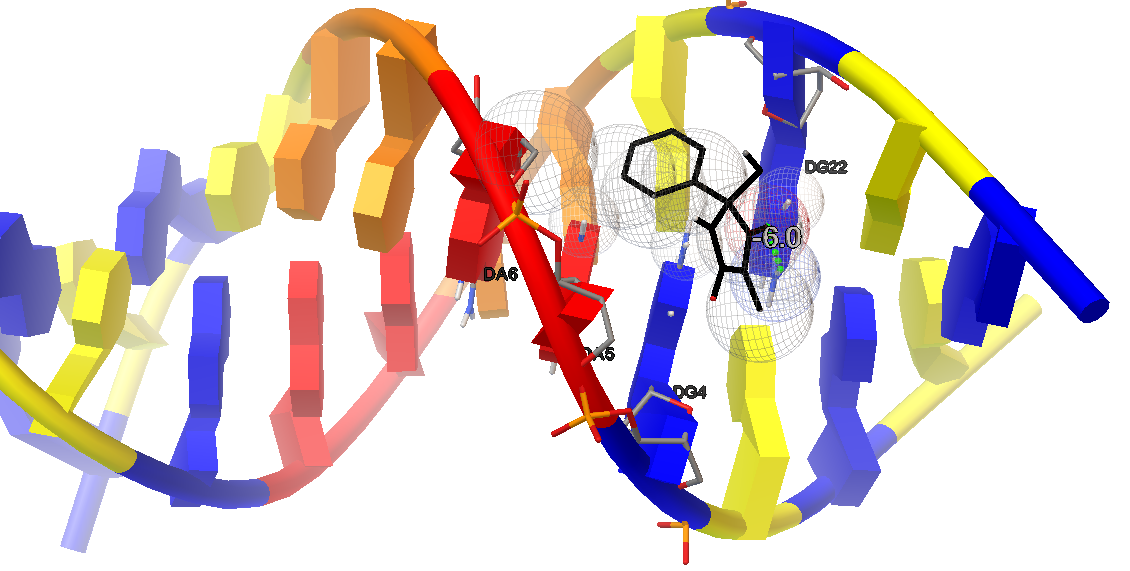
\includegraphics[width=0.8\linewidth]{mephenytoin_ribbon_9.png}
			\caption{\centering The hydrogen bonding interaction \linebreak between Mephenytoin and B-DNA.}
			\label{fig:mph_ribbon}
		\end{figure}
		\vspace{-1.5em}
		\scriptsize
		\begin{table}
			\tiny
			\begin{tabular}{ c | c c c } 
				\multirow{2}{7.6em}{\centering \textbf{Close interactions with B-DNA}}&\multicolumn{3}{c}{\multirow{2}{10em}{\centering DA5, DA6, DG22, DG4}}\\
				&&&\\
				\hline
				\multirow{6}{7em}{\centering \textbf{Hydrogen bonds (Angstrom Å) with B-DNA}}&\multirow{2}{6em}{\centering \textbf{Donor Atom}}&\multirow{2}{4em}{\centering \textbf{Acceptor Atom}}&\multirow{2}{5em}{\centering \textbf{Bond Length (Å)}}\\
				&&&\\
				\cline{2-4}
				&\multirow{2}{6em}{\centering H21 of DG22 (Chain B)}&\multirow{2}{6em}{\centering O2 of Mephenytoin}&\multirow{2}{2em}{\centering 2.1}\\
				&&&\\
				\cline{2-4}
				&\multirow{2}{6em}{\centering H3 of DG22 (Chain B)}&\multirow{2}{6em}{\centering O2 of Mephenytoin}&\multirow{2}{2em}{\centering 2.3}\\
				&&&\\
			\end{tabular}
			\caption{\centering{The close and hydrogen bonds \linebreak between Mephenytoin and B-DNA.}}
		\end{table}
	\end{column}
	\hspace{-1em}
	\begin{column}{0.55\linewidth}
		\centering
		\scriptsize
		\begin{figure}
			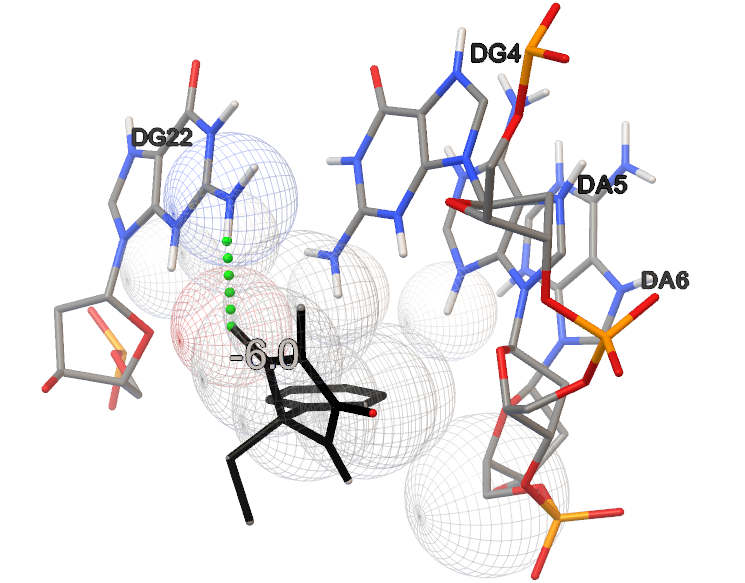
\includegraphics[width=\linewidth]{mephenytoin_yakin_1.png}
			\caption{\centering The close interaction and
				binding affinity \linebreak between Mephenytoin and B-DNA.}
			\label{fig:mph_close}
		\end{figure}
	\end{column}
\end{columns}
	\end{frame}
	\begin{frame}
		\frametitle{Docking results of Ethotoin}
\begin{columns}
	\begin{column}{0.6\linewidth}
		\begin{figure}
			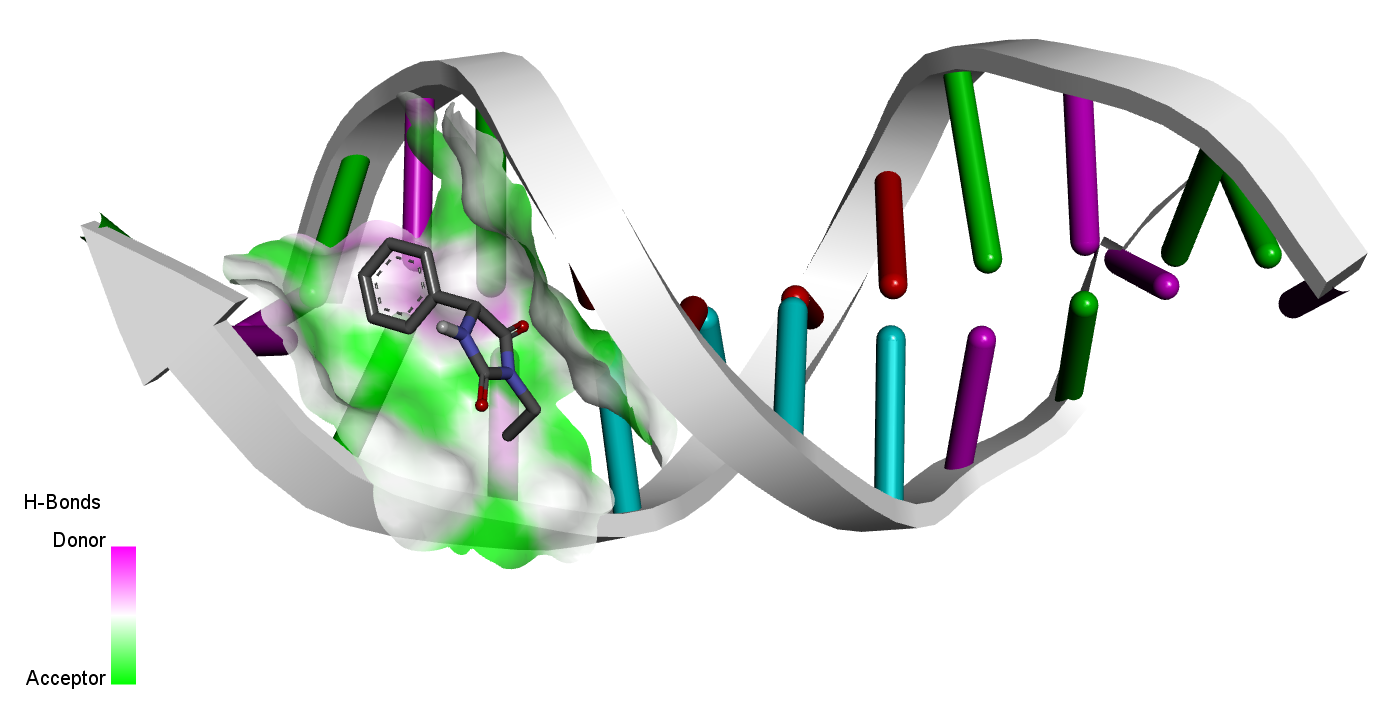
\includegraphics[width=\linewidth]{ethotoin-donor-acceptor.png}
			\caption{\centering The donor-acceptor interaction \linebreak between Ethotoin and B-DNA.}
			\label{fig:eth_donor_acceptor}
		\end{figure}
	\end{column}
	\begin{column}{0.45\linewidth}
		\centering
		\scriptsize
		\begin{table}
			\begin{tabular}{*{4}{c}}
				\hline\\[-1em]
				\multirow{2}{2em}{\centering\textbf{Mode}}&\multirow{2}{4em}{\centering\textbf{Affinity (kcal/mol)}}&\multicolumn{2}{c}{\centering\textbf{Distance from best mode}}\\
				\cline{3-4}
				&&\textbf{rmsd l.b.}&\textbf{rmsd u.b.}\\
				1&-5.8&0.000&0.000\\
				2&-5.7&2.861&5.332\\
				3&-5.7&2.603&4.023\\
				4&-5.7&1.849&5.310\\
				5&-5.7&1.750&5.199\\
				6&-5.6&2.236&5.225\\
				7&-5.4&2.600&4.039\\
				8&-5.4&3.081&5.706\\
				9&-5.3&1.431&2.061\\
				\hline
			\end{tabular}
			\caption{\centering The binding affinities and RMSD values \linebreak between Ethotoin and B-DNA.}
			\label{table:eth}
		\end{table}
	\end{column}
\end{columns}
	\end{frame}
	\begin{frame}
		\frametitle{Docking results of Ethotoin}
\begin{columns}
	\begin{column}{0.5\linewidth}
		\centering
		\vspace{-1em}
		\begin{figure}
			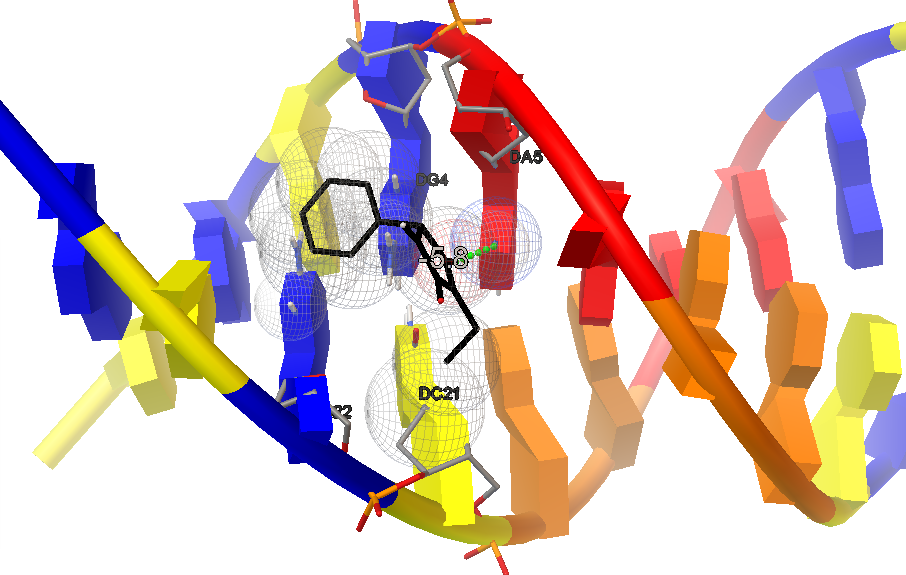
\includegraphics[width=0.7\linewidth]{ethotoin_docking_1.png}
			\caption{\centering The hydrogen bonding interaction \linebreak between Ethotoin and B-DNA.}
			\label{fig:eth_ribbon}
		\end{figure}
		\vspace{-2em}
		\scriptsize
		\begin{table}
		\tiny
		\setlength\tabcolsep{1.5pt}
		\begin{tabular}{ c | c c c } 
			\multirow{2}{7.6em}{\centering \textbf{Close interactions with B-DNA}}&\multicolumn{3}{c}{\multirow{2}{11em}{\centering DA5, DC21, DG22, DG4}}\\
			&&&\\
			\hline
			\multirow{8}{7em}{\centering \textbf{Hydrogen bonds (Angstrom Å) with B-DNA}}&\multirow{2}{6em}{\centering \textbf{Donor Atom}}&\multirow{2}{4em}{\centering \textbf{Acceptor Atom}}&\multirow{2}{5em}{\centering \textbf{Bond Length (Å)}}\\
			&&&\\
			\cline{2-4}
			&\multirow{2}{6em}{\centering H22 of DG4 (Chain A)}&\multirow{2}{6em}{\centering O2 of Ethotoin}&\multirow{2}{2em}{\centering 2.8}\\
			&&&\\
			\cline{2-4}
			&\multirow{2}{6em}{\centering H21 of DG4 (Chain A)}&\multirow{2}{6em}{\centering O2 of Ethotoin}&\multirow{2}{2em}{\centering 3.2}\\
			&&&\\
			\cline{2-4}
			&\multirow{2}{6em}{\centering H3 of DA5 (Chain A)}&\multirow{2}{6em}{\centering O2 of Ethotoin}&\multirow{2}{2em}{\centering 1.9}\\
			&&&\\
		\end{tabular}
		\caption{\centering{The close and hydrogen bonds \linebreak between Ethotoin and B-DNA.}}
		\end{table}
	\end{column}
	\hspace{-2em}
	\begin{column}{0.6\linewidth}
		\centering
		\begin{figure}
			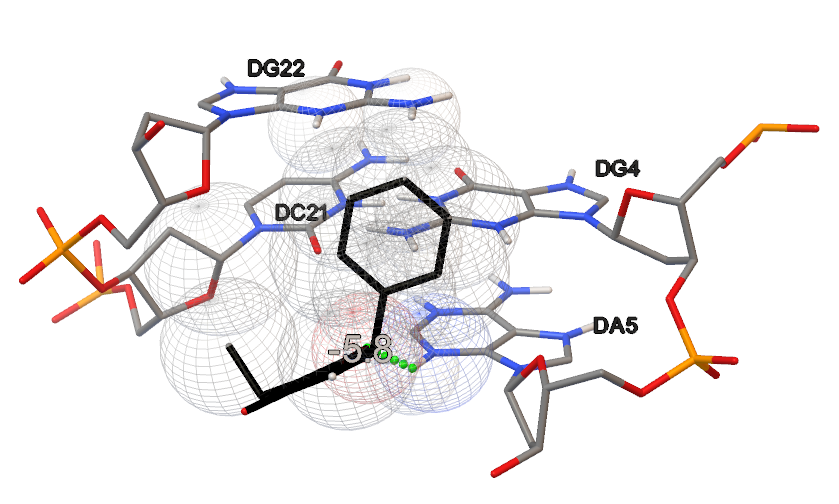
\includegraphics[width=\linewidth]{ethotoin_yakin_5.png}
			\caption{\centering The close interaction and
				binding affinity \linebreak between Ethotoin and B-DNA.}
			\label{fig:eth_close}
		\end{figure}
	\end{column}
\end{columns}
	\end{frame}
	\begin{frame}
		\scriptsize
		\bibliographystyle{unsrt}
		\bibliography{../../can_bibtex}
	\end{frame}
	\begin{frame}
		\centering \Huge Thank you for your attention.
	\end{frame}
\end{document}